\documentclass[semifinal,survey]{cpecmu}

%% This is a sample document demonstrating how to use the CPECMU
%% project template. If you are having trouble, see "cpecmu.pdf" for
%% documentation.

\projectNo{S021-2}
\acadyear{2021}

\titleTH{บีว่า: เว็บแอพพลิเคชั่นสำหรับแนะนำการเข้าใช้อาคารด้วยคำสั่งเสียงและตอบกลับด้วยเสียง}
\titleEN{BEVA: Building Enter with Voice Assistant}

\author{นายวิศรุต ติ๊บบุ่ง}{Wisarut tipbung}{620610807}

\cpeadvisor{paskorn}
\cpecommittee{kampol}
\cpecommittee{yuthapong}

%% Some possible packages to include:
\usepackage[final]{graphicx} % for including graphics

%% Add bookmarks and hyperlinks in the document.
\PassOptionsToPackage{hyphens}{url}
\usepackage[colorlinks=true,allcolors=Blue4,citecolor=red,linktoc=all]{hyperref}
\def\UrlLeft#1\UrlRight{$#1$}

%% Needed just by this example, but maybe not by most reports
\usepackage{afterpage} % for outputting
\usepackage{pdflscape} % for landscape figures and tables. 

%% Some other useful packages. Look these up to find out how to use
%% them.
% \usepackage{natbib}    % for author-year citation styles
% \usepackage{txfonts}
% \usepackage{appendix}  % for appendices on a per-chapter basis
% \usepackage{xtab}      % for tables that go over multiple pages
% \usepackage{subfigure} % for subfigures within a figure
% \usepackage{pstricks,pdftricks} % for access to special PostScript and PDF commands
% \usepackage{nomencl}   % if you have a list of abbreviations

%% if you're having problems with overfull boxes, you may need to increase
%% the tolerance to 9999
% \tolerance=9999

\bibliographystyle{plain}
% \bibliographystyle{IEEEbib}

% \renewcommand{\topfraction}{0.85}
% \renewcommand{\textfraction}{0.1}
% \renewcommand{\floatpagefraction}{0.75}

%% Example for glossary entry
%% Need to use glossary option
%% See glossaries package for complete documentation.
\ifglossary
  \newglossaryentry{lorem ipsum}{
    name=lorem ipsum,
    description={derived from Latin dolorem ipsum, translated as ``pain itself''}
  }
\fi

%% Uncomment this command to preview only specified LaTeX file(s)
%% imported with \include command below.
%% Any other file imported via \include but not specified here will not
%% be previewed.
%% Useful if your report is large, as you might not want to build
%% the entire file when editing a certain part of your report.
% \includeonly{chapters/intro,chapters/background}

\begin{document}
\maketitle
\makesignature

\ifproject
\begin{abstractTH}
การเขียนรายงานเป็นส่วนหนึ่งของการทำโครงงานวิศวกรรมคอมพิวเตอร์
เพื่อโครงงานนี้มุ่งเน้นการพัฒนา chatbot ที่สามารถทำงานได้ผ่านเสียงของผู้ใช้งานเพื่อให้ความสะดวกสบายในการค้นหาเส้นทางภายในอาคาร
รวมถึงข้อมูลอื่น ๆ เช่น เวลา สภาพอากาศ และตำแหน่งของอาจารย์ โดยใช้เทคโนโลยี Text-to-Speech (TTS) ในการสื่อสารกับผู้ใช้งาน
วัตถุประสงค์ของโครงงานนี้คือ เพิ่มประสิทธิภาพการเข้าถึงข้อมูล ให้ข้อมูลเพิ่มเติมเช่นเวลา, สภาพอากาศ, และตำแหน่งของอาจารย์ ช่วยผู้ใช้งานในการค้นหาเส้นทางภายในอาคาร
และประยุกต์ใช้ Text-to-Speech (TTS) เพื่อสร้างเสียงสังเคราะห์ที่สื่อสารกับผู้ใช้งาน โครงงานนี้จัดทำขึ้นโดยนายวิศรุต ติ๊บบุ่ง และมีขอบเขตที่ ทำที่ตึก 30 ปี
ในมหาวิทยาลัยเชียงใหม่ ต้องเชื่อมต่อ Internet และรองรับการใช้งานผ่าน browser เท่านั้น ต้องใช้คอมพิวเตอร์ในการใช้งานเว็บไซต์
และรองรับการสนทนาและตอบคำถามภาษาไทยเท่านั้น โครงการนี้คาดว่าจะช่วยให้บริการด้านเส้นทางภายในอาคารและลดความเสี่ยงต่อการแพร่ระบาดของเชื้อโควิด-19
โดยลดการใช้งานมนุษย์และการใกล้ชิดกับผู้อื่น เมื่อโครงการสำเร็จ จะสามารถให้ประโยชน์ในด้านการสนับสนุนความสะดวกสบายในการเข้าถึงข้อมูล ลดการใช้ทรัพยากรมนุษย์
และป้องกันการแพร่ระบาดของเชื้อโควิด-19 โดยสามารถนำไปติดตั้งที่อาคารต่าง ๆ ได้ในอนาคต
\end{abstractTH}

\begin{abstract}
  Writing a report is an integral part of working on a computer engineering project.
  This project focuses on the development of a chatbot that can operate through user's voice input,
  providing convenience in searching for routes within buildings, as well as other information such as time,
  weather conditions, and the location of professors. This is achieved using Text-to-Speech (TTS) technology
  to communicate with users. The objective of this project is to increase the efficiency of accessing
  information, provide additional details such as time, weather, and the location of professors, assist
  users in finding routes within buildings, and apply Text-to-Speech (TTS) technology to create synthesized
  voices that communicate with users. This project is carried out by Mr. Wisarut Tibbung and is limited to
  the 30-year-old building at Chiang Mai University. It requires an internet connection and supports usage
  via a browser only, using a computer for website access, and supports Thai language conversation and question
  answering only. This project is expected to help provide services related to routes within buildings while
  reducing the risk of spreading COVID-19 by minimizing human interaction and close contact with others.
  Once completed, the project will benefit users by supporting their convenience in accessing information,
  reducing human resource usage, and preventing the spread of COVID-19, with the potential to be installed in
  various buildings in the future.
\end{abstract}

\iffalse
\begin{dedication}
This document is dedicated to all Chiang Mai University students.

Dedication page is optional.
\end{dedication}
\fi % \iffalse

\begin{acknowledgments}
ในโครงงานฉบับนี้ สำเร็จลุล่วงได้อย่างสมบูรณ์ด้วยความกรุณาอย่างยิ่งจาก
ผศ.ดร.ภาสกร แช่มประเสริฐ ที่ได้สละเวลาอันมีค่าแก่ผู้จัดทำโดยให้คำปรึกษาและแนะนำตลอดจน
ตรวจทานแก้ไขข้อบกพร่องต่างๆด้วยความเอาใจใส่เป็นอย่างยิ่ง จนโครงงานฉบับนี้สำเร็จสมบูรณ์
ลุล่วงได้ด้วยดีผู้จัดทำขอกราบขอบพระคุณเป็นอย่างสูงไว้ ณ ที่นี้ จากใจจริง
ขอขอบคุณ อ.ดร.ชินวัตร อิศราดิสัยกุล ที่ได้กรุณาให้คำแนะนำและให้ข้อมูลสำหรับการทำโครงงาน
ขอขอบคุณ รศ.ดร.อัญญา อาภาวัชรุตม์ วีระประพันธ์ ที่ได้กรุณาให้คำแนะนำและแนวมางในการปรับปรุงโครงงานชิ้นนี้
ขอขอบคุณ ผศ.ดร.ยุทธพงษ์ สมจิต ที่ได้กรุณาให้คำแนะนำและแนวมางในการปรับปรุงโครงงานชิ้นนี้

\acksign{2023}{3}{31}
\end{acknowledgments}%
\fi % \ifproject

\contentspage

\ifproject
\figurelistpage

\tablelistpage
\fi % \ifproject

% \abbrlist % this page is optional

% \symlist % this page is optional

% \preface % this section is optional


\pagestyle{empty}\cleardoublepage
\normalspacing \setcounter{page}{1} \pagenumbering{arabic} \pagestyle{cpecmu}

\chapter{\ifenglish Introduction\else บทนำ\fi}

\section{\ifenglish Project rationale\else ที่มาของโครงงาน\fi}
อาคารหลายๆแห่งในตอนนี้นั้นบางอาคารใหญ่บางอาคารเล็กและยิ่งอาคารใหญ่ ยิ่งถ้าเลยมาครั้งแรกแล้วละก็ยิ่งทำให้หาห้องลำบาก
ไม่ว่าจะเป็นห้องเรียน ห้องประชุม หรือแม้กระทั้งห้องน้ำนั้นก็ยังหาลำบาก ด้วยเหตุนี้ก็ยังจะทำให้คนที่เข้ามาใช้หรือติดต่อ
งานต่างๆนั้นหาทางไปให้ถึงห้องที่ตัวเองต้องการนั้นยากเพราะไม่เคยมา ถึงจะมีแผนที่ภายในอาคารแต่ก็ยังอ่านยากอยู่ดี เพราะเหตุ
นี้จีงเป็นที่มาของโครงการนี้ BEVA (Building Enter with Voice Assistant) หรือในชื่อภาษาไทยก็คือ
เว็บแอพพลิเคชั่นสำหรับแนะนำการเข้าใช้อาคารด้วยคำสั่งเสียงและตอบกลับด้วยเสียง นั้นสร้างขึ้นมาเพื่ออำนวนความสะดวกให้กับ
ผู้ใช้งานอาคารในการหาห้องต่างๆ โดยไม่ต้องเสียเวลามาไล่หาห้องในแผนที่ทีละชั้น

\section{\ifenglish Objectives\else วัตถุประสงค์ของโครงงาน\fi}
\begin{enumerate}
    \item เพื่อพัฒนาระบบแนะนำการเข้าใช้ห้องต่างๆภายในอาคาร แบบ real-time
    \item เพื่อลดการใช้มนุษย์โดยให้ BEVA เข้าไปทำงานแทนในส่วนของการตอบคำถามประเภทเส้นทาง
    และรวมไปถึงถามเวลาเข้าใช้ห้องประชุมหรือห้องเรียนต่างๆในสถานการณ์ที่เชื้อ covid-19 กำลังระบาด
    \item เก็บสถิติผู้เข้าใช้อาคารเพื่อนำไปใช้ในการพัฒนาการให้บริการของอาคารนั้นๆในอนาคต
\end{enumerate}

\section{\ifenglish Project scope\else ขอบเขตของโครงงาน\fi}
\begin{enumerate}
    \item ลองทำที่ตึก ITSC
    \item ต้องเชื่อมต่อ Internet
    \item ต้องใช้คอมพิวเตอร์ในการเปิดเว็บ
    \item รองรับเฉพาะภาษาไทย
    \item ตอบคำถามได้ที่ละ 1 คำถามโดยแต่ละคำถามอาจจะมีความตต่อเนื่องกัน
\end{enumerate}

\subsection{\ifenglish Hardware scope\else ขอบเขตด้านฮาร์ดแวร์\fi}
\begin{enumerate}
    \item ใช้คอมพิวเตอร์ในการเปิด Web browser
    \item ใช้จอในการแสดงผลข้อมูลและเส้นทางการเดินทาง
    \item ใช้ไมโคโฟนในการรับสัญญาณเสียงจากผู้ใช้งาน
    \item ใช้ลำโพงเพื่อตอบกลับผู้ใช้ด้วยเสียงพูด
\end{enumerate}

\subsection{\ifenglish Software scope\else ขอบเขตด้านซอฟต์แวร์\fi}
\begin{enumerate}
    \item OS: Windows 10 or Linux.
    \item Browser: Google Chrome, Firefox or Edge.
\end{enumerate}

\section{\ifenglish Expected outcomes\else ประโยชน์ที่ได้รับ\fi}
เป็นโปรแกรมที่ช่วยอำนวยความสะดวกผู้ใช้ในด้านที่สามารถสอบถามเส้นทาง สถิติและสภาพอากาศ 
ได้ทันทีโดยไม่ต้องเข้าเว็บหาหรือสอบถามที่ประชาสัมพันธ์และในด้านของผู้ให้บริการการหรือทางเจ้าของอาคาร
ก็ไม่ต้องจัดคนมาคอยให้บริการในส่วนการแนะนำเส้นทางการเข้าใช้ห้องต่างๆภายในอาคารอีกด้วย

\section{\ifenglish Software technology\else เทคโนโลยีด้านซอฟต์แวร์\fi}
\begin{enumerate}
    \item React: library ที่ใช้ในการพัฒนา
    \item JS: ภาษาที่ใช้ในการพัฒนา
    \item Node.js: คือสภาพแวดล้อมการทำงานของภาษา JavaScript
    \item Google TTS: API ที่ใช้ในการแปลคำตอบไปเป็นเสียงเพื่อให้ผู้ใช้ฟัง
    \item Google STT: API ที่ใช้ในการแปลเสียงของผู้ใช้ไปเป็นตัวอักษรเพื่อส่งเข้าโปรแกรม
    \item OpenWeatherMap: API ที่ใช้ในการดึงข้อมูลสภาพอากาศ
    \item Google Dialogflow: เครื่องมือสำหรับสร้าง chatbot
    \item Google Firestore: database สำหรับเก็บข้อมูลแผนที่และข้อมูลอื่นๆ
\end{enumerate}

\section{\ifenglish Project plan\else แผนการดำเนินงาน\fi}

\begin{plan}{11}{2021}{11}{2022}
    \planitem{11}{2021}{10}{2022}{ศึกษาค้นคว้า}
    \planitem{1}{2022}{2}{2022}{เชื่อม API กับระบบ}
    \planitem{3}{2022}{3}{2022}{เตรียมแผนที่ภายในอาคาร}
    \planitem{3}{2022}{3}{2022}{ทำ video แนะนำเส้นทาง}
    \planitem{4}{2022}{4}{2022}{test ระบบครั้งที่ 1}
    \planitem{5}{2022}{5}{2022}{เตรียมข้อมูลสำหรับ train model}
    \planitem{5}{2022}{6}{2022}{train และ tune model}
    \planitem{6}{2022}{6}{2022}{test ระบบครั้งที่ 2}
    \planitem{7}{2022}{11}{2022}{นำระบบที่พัฒนาสำเร็จและผ่านการทดสอบแล้วไปทดลองใช้งาน}
\end{plan}

\begin{plan}{12}{2022}{12}{2023}
    \planitem{12}{2022}{2}{2023}{ประเมินผลและสำรวจความคิดเห็นของผู้ใช้}
\end{plan}

\section{\ifenglish Roles and responsibilities\else บทบาทและความรับผิดชอบ\fi}
โครงงานนี้ได้จัดทำขึ้นโดยผู้จัดทำเพียงคนเดียวคือ นาย วิศรุต ติ๊บบุ่ง

\section{\ifenglish%
Impacts of this project on society, health, safety, legal, and cultural issues
\else%
ผลกระทบด้านสังคม สุขภาพ ความปลอดภัย กฎหมาย และวัฒนธรรม
\fi}
ถ้าหากโครงการนี้สำเร็จอาจจะเกิดผลกระทบด้านความปลอดภัยและสุขภาพเป็นหลักเพราะว่า โครงการของเราสามารถเชื่อต่อกับ api ที่เกี่ยวกับ
การทำ face recognition เพื่อที่จะสามารถรับรู้ได้ว่าคนนี้คือใครและสามารถบันทึกข้อมูลของคนนั้นเก็บไว้บน cloud เพื่อช่วยในการรักษาความปลอดภัย
ของผู้เข้าใช่อาคารได้ซึ่งเป็นหนึ่งใน use caseของโครงการนี้ ส่วนทางด้านของสุขภาพ นั้นก็เป็นอีกหนึ่งเป้าหมายของเราเพื่อที่จะลดการใช้ทรัพยากรมนุษย์ 
ในสถานะการที่มีการแพร่ระบาดของ virus covid-19 เราจะนำโครงการนี้ไปติดตั้งที่อาคารต่างๆเพื่อให้บริการด้านเส้นทางภายในอาคารและลดความเสี่ยงต่อ
การเกิดอันตรายจากการที่มีการใกล้ชิดกับผู้อื่น พร้อมทั้งยังช่วยลดการแพร่ระบาดอีกด้วย
\chapter{\ifenglish Background Knowledge and Theory\else ทฤษฎีที่เกี่ยวข้อง\fi}

โครงการนี้เป็นการสร้างระบบตอบรับแบบอัตโนมัติโดยรับคำสั่งผ่านทางเสียงและตอบกลับด้วยเสียงออกมาทันที
โดยจะมีตัวกลางในการเชื่อมต่อและเป็นหัวใจหลักของโครงงานนี้ นั้นก็คือ dialogflow ซึ้งเป็น API AI
ที่จะเข้ามาช่วยในการสร้างระบบตอบรับแบบอัตโนมัติและเพื่อให้ dialogflow ที่รับ input เป็นข้อความเข้าใจ
คำสั่งที่ผู้ใช้พูดเราจำเป็นที่จะต้องมี API อีกตัวเข้ามาช่วย นั้นก็คือ Google Speech-To-Text ซึ้งเป็น API
ที่จะรับเสียงที่ผู้ใช้พูดออกมาแล้วแปลงเป็นข้อความเพื่อส่งให้ dialogflow เข้าใจและตอบกลับออก ซึ่งคำตอบของ
dialogflow ก็จะเป็นข้อความเพราะฉนั้นอีกสื่งที่จะขาดไปไม่ได้เลยคือ google Text-To-Speech เพื่อที่จะแปลง
คำตอบของ agent ให้กลายเป็นเสียงเพื่อที่ทำให้ผู้ใช้ได้ยินคำตอบของ agent โดยลายละเอียดทีของ API แต่ละตัวที่ใช้เป็นดังนี้

\section{เครื่องมือที่ใช้ในการพัฒนา}
\subsection{Dialogflow}
Dialogflow หรือ Api.ai เป็น product ที่ถูกพัฒนาขึ้นโดย Speaktoit ถูก Google ซื้อ และนำไปพัฒนาต่อยอดในปี
2016 และพึ่งเปลี่ยนชื่อมาเป็น Dialogflow โดยตัว Dialogflow ใช้เทคนิคด้าน Machine Learning และ natural language
processing (NLP) ทำให้เข้าใจการสนทนาของมนุษย์และสามารถในไปใช้ได้หลากหลายรูปแบบ และ Dialogflow ยังสามารถเชื่อมต่อกับ
Facebook, Twitter และอื่นๆได้ง่าย มันยังสามารถเชื่อมต่อกับ Google Cloud Speech-to-Text ได้ด้วย ซึ่งที่ผ่านมา
Dialogflow เป็นเครื่องมือสำคัญในการสร้างบทสนทนาที่ใช้บน Google Assistant~\cite{df-doc}

\subsection{Google Speech-To-Text}
API Google Speech-To-Text (gSTT) ของ Google เป็นอีกหนึ่งตัวเลือกที่ดีในการรวมการจดจำเสียงเข้ากับเว็ปแอปพลิเคชัน
โดยหลักการทำงานของ STT คือการรับเสียงเข้าไปประมวลผลและตอบกลับออกมาเป็นข้อความ~\cite{gstt-doc}

\subsection{Google Text-To-Speech}
เช่นเดียวกับ Google Speech-To-Text Google Text-To-Speech นั้นเป็นบริการของ Google Cloud platform
สำหรับการแปลงข้อความให้กลายเป็นเสียงพูด เพื่อตอบโต้กับผู้ใช้งานทำให้ผู้ใช้งานนั้นรู้สึกเหมือนได้คุยกับคนจริงๆ~\cite{gtts-doc}

\subsection{Google Firebase}
Firebase คือ Platform ที่รวบรวมเครื่องมือต่าง ๆ สำหรับการจัดการในส่วนของ Backend หรือ Server side
ซึ่งทำให้สามารถสร้าง Web Application ได้อย่างมีประสิทธิภาพ และยังลดเวลาและค่าใช้จ่ายของการทำ Server side
หรือการวิเคราะห์ข้อมูลให้อีกด้วย โดยมีทั้งเครื่องมือที่ฟรี และเครื่องมีที่มีค่าใช้จ่าย (สำหรับการ Scale) ซึ่งบริการหลักๆของ
Firebase ที่เราใช้จะมีดังนี้~\cite{fs-doc}

\begin{enumerate}
  \item Cloud Storage คือ บริการจัดเก็บไฟล์ข้อมูลในระบบ cloud ที่มีความปลอดภัยสูง เพื่อรองรับการดาวน์โหลดและอัพโหลดไฟล์ข้อมูลขนาดใหญ่
  \item Cloud Firestore คือ บริการทางด้าน Database ที่เป็นลักษณะเป็น NoSQL โดนจะจัดกับข้อมูลในรูปแบบ JSON files format
\end{enumerate}

\subsection{React}
React คือ JavaScript Library ที่ทีม Facebook เป็นคนพัฒนาขึ้นมา และเปิดให้คนทั่วไปนำมาใช้ฟรี ซึ่งเว็บไซต์ในปัจจุบันของ
Facebook.com ก็ใช้ React อยู่เช่นกัน สรุปคือ โดยมีคอนเซปต์ที่ต้องรู้เพื่อเขียน React หลักๆ 3 Concept เท่านั้นเอง~\cite{react-doc}

\begin{enumerate}
  \item Component: ส่วนต่าง ๆ ในเว็บเราจะมองเป็น Component
  \item State: ข้อมูลที่อยู่ใน Component แต่ละชิ้น เราเรียกว่า State
  \item Props: ข้อมูลที่ถูกส่งต่อจาก Component ชั้นบนลงไปชั้นล่าง เราเรียกว่า Props (Properties)
\end{enumerate}


\subsection{JS}
JavaScript คือ ภาษาคอมพิวเตอร์สำหรับการเขียนโปรแกรมบนระบบอินเทอร์เน็ต ที่กำลังได้รับความนิยมอย่างสูง Java JavaScript
เป็น ภาษาสคริปต์เชิงวัตถุ ที่เรียกกันว่า "สคริปต์" (script) ซึ่งในการสร้างและพัฒนาเว็บไซต์ (ใช่ร่วมกับ HTML) เพื่อให้เว็บไซต์ของ
เราดูมีการเคลื่อนไหว สามารถตอบสนองผู้ใช้งานได้มากขึ้น ซึ่งมีวิธีการทำงานในลักษณะ "แปลความและดำเนินงานไปทีละคำสั่ง"
(interpret) หรือเรียกว่า อ็อบเจ็กโอเรียลเต็ด (Object Oriented Programming) ที่มีเป้าหมายในการ ออกแบบและพัฒนา
โปรแกรมในระบบอินเทอร์เน็ต สำหรับผู้เขียนด้วยภาษา HTML สามารถทำงานข้ามแพลตฟอร์มได้ โดยทำงานร่วมกับ ภาษา HTML และภาษา
Java ได้ทั้งทางฝั่งไคลเอนต์ (Client) และ ทางฝั่งเซิร์ฟเวอร์ (Server)~\cite{js-doc}

\subsection{Express}
Express.js เป็น Web Application Framework ที่ได้รับความนิยมมากสำหรับการทำงานบน platform ของ Node.js
ซึ่งเป็น Server ตัวหนึ่ง โดยทั้ง Express.js และ Node.js ต่างก็ใช้ภาษา Javascript ในการพัฒนา ถ้าเป็น Web
Application Framework ในสมัยก่อน คนที่พัฒนาจะต้องมีความรู้มากกว่า 1 ภาษา ภาษาที่ทำงานทางฝั่ง Server อย่าง PHP
หรือ ASP และภาษาที่ทำงานทางฝั่ง Client อย่าง JavaScript เพื่อลดความยุ่งยากรวมถึงเวลาในการต้องเรียน รู้หลายๆ ภาษาทำให้เกิด
Node.js กับ Express.js เพียงแค่มีความรู้ Javascript ก็สามารถเขียนได้ทั้ง Server และ Client และเนื่องจากใช้
Javascript ในการพัฒนาจึงทำให้ตัว Express นั้นตอบสนองเร็วมาก~\cite{express-doc}

\subsection{OpenWeatherMap}
OpenWeatherMap คือผู้ให้บริการ API ที่ให้บริการดึงข้อมูลสภาพอากาศทั่วโลก ซึ่งให้ข้อมูลผ่าน API ซึ่งรวมถึงข้อมูลสภาพอากาศในปัจจุบันม
พยากรณ์อากาศ ซึ่งมีทั้งรายการในปัจจุบัน และข้อมูลสภาพอากาศในอดีตสำหรับแต่ละพื่นที่บนโลก โดยบริษัทได้จัดทำการคาดการณ์ปริมาณน้ำฝน
แบบไฮเปอร์โลคัลแบบนาทีต่อนาทีสำหรับแต่ละสถานที่ โดยอาศัยข้อมูลอากาศจากกรมอุตุนิยมวิทยาและข้อมูลจากสถานีตรวจอากาศสนามบิน,
สถานีเรดาร์ภาคพื้นดิน, ดาวเทียมตรวจสภาพอากาศ, ดาวเทียมสำรวจระยะไกล METAR และสถานีตรวจอากาศอัตโนมัติทั่วโลก~\cite{openweather-doc}


\section{ทฤษฎีการออกแบบ UX/UI}
การออกแบบแอพพลิเคชั่นและเว็บไซต์ มีเรื่องมากมายที่ทำให้ดีไซน์เนอร์ปวดหัว เพราะมันไม่ใช่แค่ความสวยงาม แต่คือการออกแบบเพื่อตอบ
โจทย์การใช้งานของผู้ใช้ให้มากที่สุด และสิ่งที่เราจะพูดถึงในบทความนี้คือ “ลายแทง สำหรับนักออกแบบ” ก่อนลงมือพัฒนาจริง ในการออก
แบบ UI ที่ดี ต้องคำนึงถึงองค์ประกอบดังนี้
\begin{enumerate}
  \item Visibility คือ มีความชัดเจนที่จะบ่งบอกถึงเอกลักษณ์เฉพาะตัวของแอพ โดยคำนึงการใช้งาน และมี Concept ที่ชัดเจน
  \item Development ต้องคำนึงถึง ความสามารถในการปรับแต่งและข้อจำกัดของ platform เช่น การรองรับ การสร้างต้นแบบที่รวดเร็ว, มีคลังข้อมูล และมีชุดเครื่องมือที่รองรับ เพื่อที่จะสามารถต่อยอดและพัฒนาต่อไปได้
  \item Colors การเลือกใช้สีที่ดี จะช่วยให้ผู้ใช้เกิดการจดจำที่ดียิ่งขึ้นมากกว่าการใช้เพียงแค่สีขาว-ดำ อีกทั้งรวมถึงการเพิ่มประสิทธิภาพและดึงดูดผู้ใช้งานอีกด้วย นอกจากนั้นประโยชน์ของการใช้สียังรวมไปถึง
  \item Animation การที่มีอนิเมชั่นเพื่อที่จะดึงดูดให้ผู้ใช้ให้มาใช้แอพที่ video ดีกว่าการใช้แผนทีแบบเดิมๆ
\end{enumerate}

\section{\ifenglish%
    \ifcpe CPE \else ISNE \fi knowledge used, applied, or integrated in this project
  \else%
    ความรู้ตามหลักสูตรซึ่งถูกนำมาใช้หรือบูรณาการในโครงงาน
  \fi
}
ความรู้จากวิชา พื้นฐานของระบบฐานข้อมูล (261342) และวิชา ปฏิบัติการระบบฐานข้อมูล
(261343) ได้ถูกนำมาใช้ต่อยอดเพื่อศึกษาขั้นตอนวิธีการจัดการฐานข้อมูล เพื่อเก็บข้อมูลแผนที่และ video สำหรับ
นำมาใช้แสดงผลที่หน้า Web Application ของโครงงาน

\section{\ifenglish%
    Extracurricular knowledge used, applied, or integrated in this project
  \else%
    ความรู้นอกหลักสูตรซึ่งถูกนำมาใช้หรือบูรณาการในโครงงาน
  \fi
}

ศึกษาวิธีการใช้สร้างและใช้งาน Dialogflow, Google TTS, Google STT , Cloud Storage 
และ Cloud Firestore ผ่านทางอินเทอร์เน็ตเพื่อสร้างระบบฝั่ง Web Server ที่จะคอยจัดการข้อมูลต่างๆ
ของแผนที่และอาจจะรวมไปถึงข้อมูลต่างๆ ข้อผู้ใช้

\chapter{\ifproject%
    \ifenglish Project Structure and Methodology\else โครงสร้างและขั้นตอนการทำงาน\fi
  \else%
    \ifenglish Project Structure\else โครงสร้างของโครงงาน\fi
  \fi
 }

ในบทนี้จะกล่าวถึงภาพรวมของ BEVA ที่จะสร้างว่ามีการใช้งานอย่างไรการทำงานของ Dialogflow ทำงานอย่างไร
พร้อมทั้งอธิบายการจัดการ database ทั้ง Cloud Storage และ Firestore ว่าวางแผนไว้อย่างไร

\makeatletter

% \renewcommand\section{\@startsection {section}{1}{\z@}%
%                                    {13.5ex \@plus -1ex \@minus -.2ex}%
%                                    {2.3ex \@plus.2ex}%
%                                    {\normalfont\large\bfseries}}

\makeatother
%\vspace{2ex}
% \titleformat{\section}{\normalfont\bfseries}{\thesection}{1em}{}
% \titlespacing*{\section}{0pt}{10ex}{0pt}

\section{โครงสร้าง}
\begin{figure}[hbt!]
  \begin{center}
    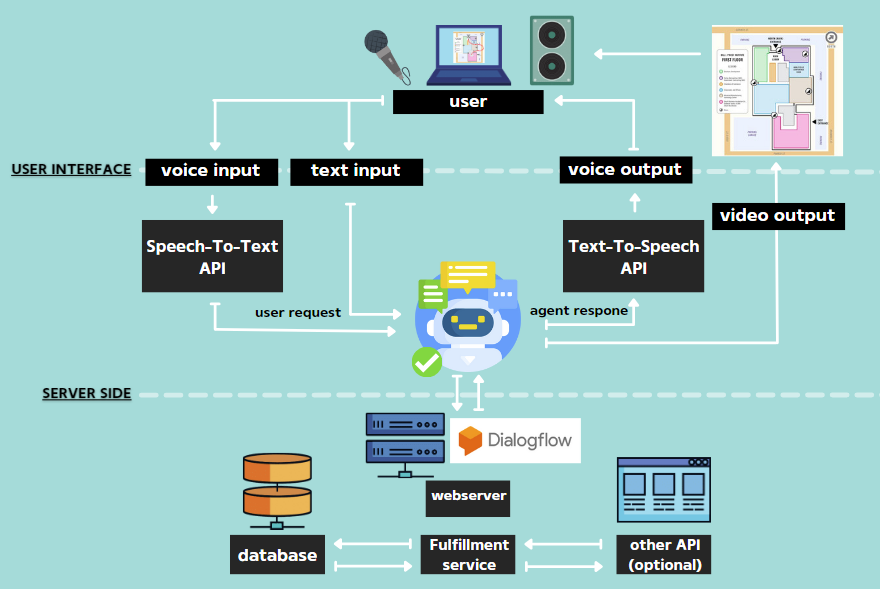
\includegraphics[width=\textwidth,keepaspectratio]{pic/overview.png}
  \end{center}
  \caption{ภาพรวมการทำงานของ BEVA}
  \label{fig:overview}
\end{figure}
โปรเจคนี้ทำการพัฒนาแชทบอทผ่าน Dialogflow ที่เชื่อมต่อกับ Web application และทำการเชื่อมต่อเขียน
โปรแกรมโดยใช้ NodeJS ดึงข้อมูลจาก Database โดยชนิดของ Database ที่ใช้เป็นแบบ NoSQL ซึ่งเมื่อผู้ใช้
ถามคำถามผ่านทางการพูดใส่ไมค์ที่อยู่บริเวณอาคาร ตัว Web จะส่ง user request Google STT ก่อนเพื่อแปลง
เสียงที่ได้รับมาให้กลายเป็นข้อความและตอบกลับมาที่เว็บหลังจากได้ตัวข้อความแล้วก็จะส่ง user request ไปยัง
Dialogflow ซึ่งคำถามที่ส่งมานั้นจะถูกแยกออกเป็น 3 กรณีนั่นคือ

\begin{enumerate}
  \item ไม่ต้องการข้อมูลจาก database หรือ API: คำตอบจะถูกส่งคืนกลับไปเป็น agent response
        ของ Dialogflow
  \item ต้องการข้อมูลจาก database: Dialogflow จะทำการส่ง API ไปที่ webhook จากนั้นจะทำการ
        ดึงข้อมูลจาก database แล้วส่งกลับไปยัง Dialogflow ในรูปแบบของ JSON เพื่อให้ Dialogflow ส่ง
        คำตอบให้ผู้ใช้งานต่อไป
  \item ต้องการข้อมูลจาก API: Dialogflow จะทำการส่ง API ไปที่ webhook จากนั้นจะทำการข้อมูล
        ซึ่ง API จะตอบกลับมาในรูปของ JSON ให้กับ Dialogflow และให้ Dialogflow ส่งคำตอบให้ผู้ใช้งานอีกที่
\end{enumerate}
\section{Database}
\subsection{รูปแบบการเก็บข้อมูลใน Cloud Firestore}
รูปแบบในการเก็บข้อมูลที่เลือกใช้จะเป็นแบบ NoSQL บน Cloud Firestore ซึ่งเราได้วางโครงสร้างไว้ดังนี้
\begin{figure}[hbt!]
  \begin{center}
    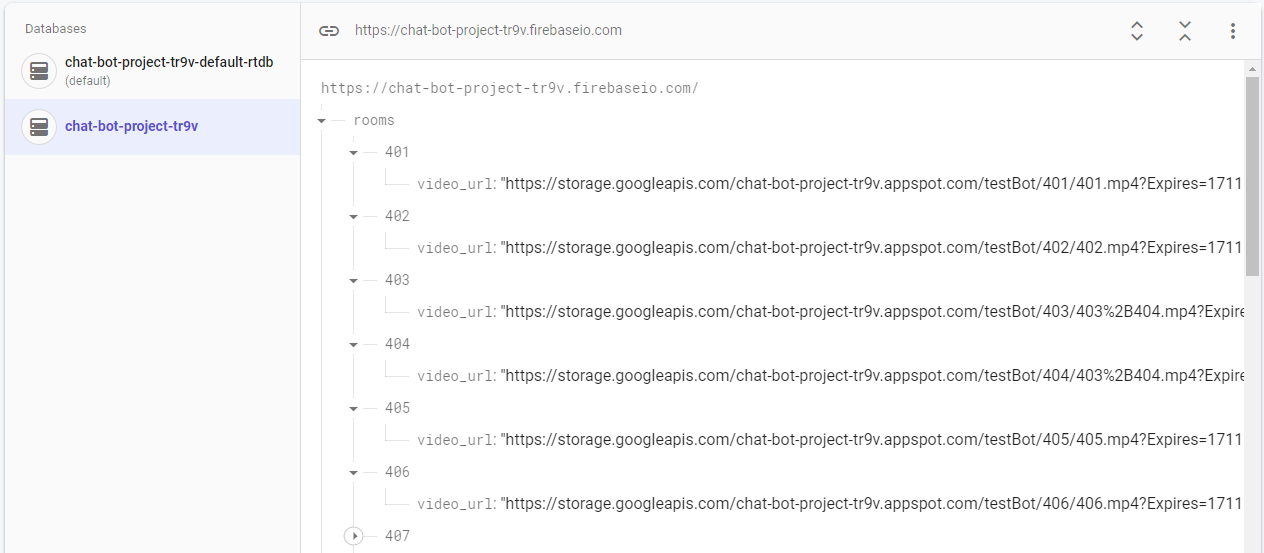
\includegraphics[width=\textwidth,keepaspectratio]{pic/database_mapPath.png}
  \end{center}
  \caption{การเก็บข้อมูลที่อยู่ของไฟล์ video แผนที่สำหรับแต่ละห้อง}
  \label{fig:db_mapPath}
\end{figure}

\subsection{รูปแบบการเก็บข้อมูลใน Cloud Storage}
รูปแบบในการเก็บข้อมูลที่อยู่บน Cloud Storage จะมีลักษณะเหมือนกับ Google Drive เราสามารถอัพโหลดไฟล์ขึ้นไปฝากไว้บน Cloud
ได้โดยบนนี้เราจะเก็บไฟล์ video ที่แสดงเส้นทางไปยังห้องต่างๆในแต่ละชั้นดังนี้
\begin{figure}[hbt!]
  \begin{center}
    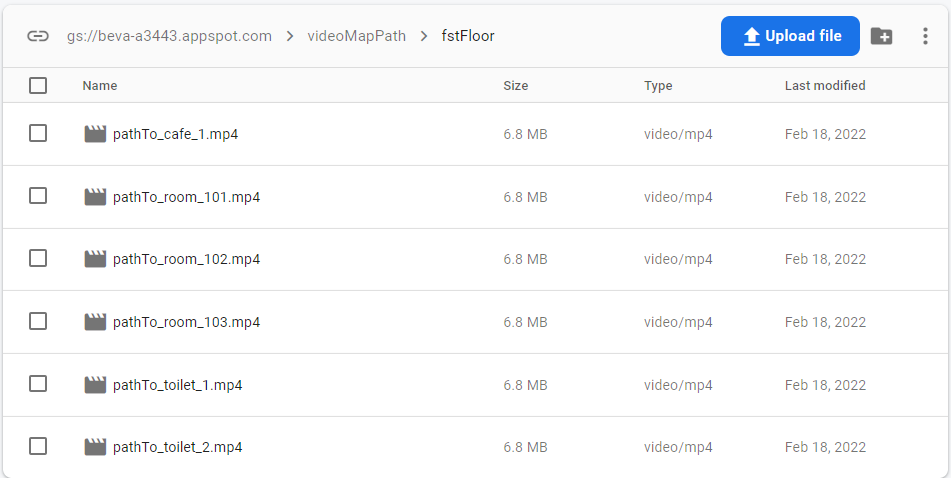
\includegraphics[width=\textwidth,keepaspectratio]{pic/db_storage.png}
  \end{center}
  \caption{การเก็บข้อมูลไฟล์ video แผนที่สำหรับแต่ละห้อง}
  \label{fig:db_storage}
\end{figure}

\begin{figure}[hbt!]
  \begin{center}
    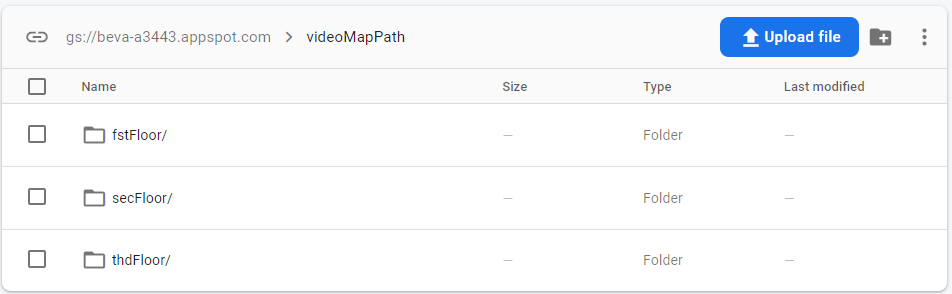
\includegraphics[width=\textwidth,keepaspectratio]{pic/db_storage_floorFolder.png}
  \end{center}
  \caption{folder สำหรับเก็บ video ของแผนที่สำหรับแต่ละห้อง}
  \label{fig:db_storage_floorFolder}
\end{figure}

\section{การทำงานของ Dialogflow}

Dialogflow ใช้เทคนิค Natural language ในการสื่อสารระหว่างคอมพิวเตอร์เเละภาษามนุษย์ จากจุดเด่นดั้งกล่าว เราจีงเลือก
Dialogflow มาเป็นตัวกลางระหว่างมนุษย์แลคอมพิวเตอร์ Chatbot~\cite{df-overview}
\subsection{การเปลี่ยน Input ให้เป็น Intent}
สามารถแบ่งออกได้เป็น 3 ขั้นตอน
\begin{enumerate}
  \item ผู้ใช้งานพิมพ์ข้อความ (Input) เข้ามา ซึ่งอาจจะเป็นชุดคำพูดหรือประโยค (Utterance)
  \item ระบบจะทำการหาใจความสำคัญที่ผู้ใช้ต้องการที่จะสื่อ (Intent) ให้กับ Chatbot มา process
  \item หลังจากระบุ Intent ได้แล้ว ระบบจะทำขั้นตอน Intent Matching เพื่อหา Response หรือการตอบกลับต่อข้อความนั้น
\end{enumerate}

\begin{figure}[hbt!]
  \begin{center}
    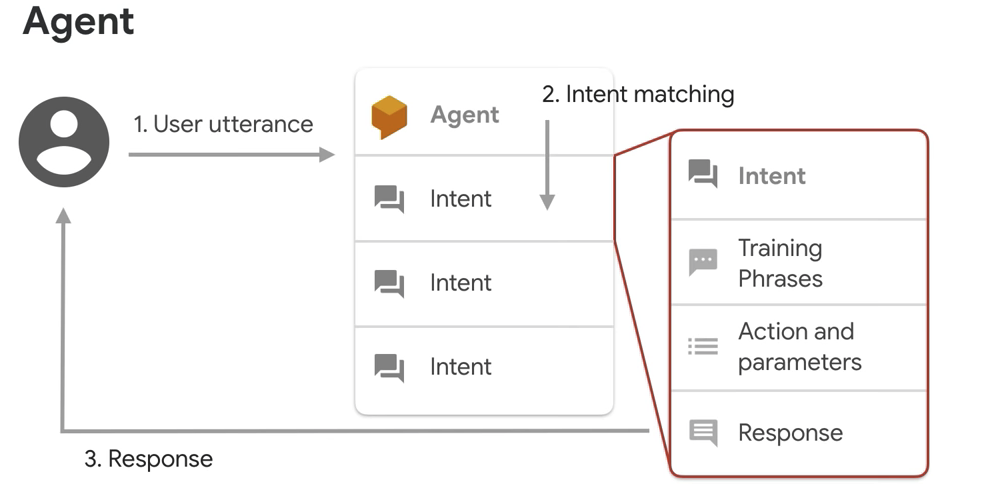
\includegraphics[width=\textwidth,keepaspectratio]{pic/df_input_intent_conventer.png}
  \end{center}
  \caption{การแปลง Input ให้เป็น Intent}
  \label{fig:df-TTI}
\end{figure}
ตัวอย่าง Utterance หรือ ชุดคำพูดหรือประโยคที่เราคาดว่าผู้ใช้งานจะต้องใช้ (Input)
\begin{center}
``Hey Bot, Can you make an appointment for me at 9 p.m.?''
\end{center}
ตัวอย่างการระบุ Intent จะเห็นได้ว่าสิ่งที่ผู้ใช้งานต้องการคือ ทำการนัดหมายที่เวลา 9 p.m. ดังนั้น 
Intent ของประโยคนี้คือ `make an appointment for me at 9 p.m.' จากนั้น Bot 
จะทำการตอบ  Reponse ที่เราได้เตรียมไว้สำหรับ Intent นี้เป็นลำดับถัดไป
\subsection{ตรวจสอบ intent และตอบกลับ}

\begin{figure}[hbt!]
  \begin{center}
    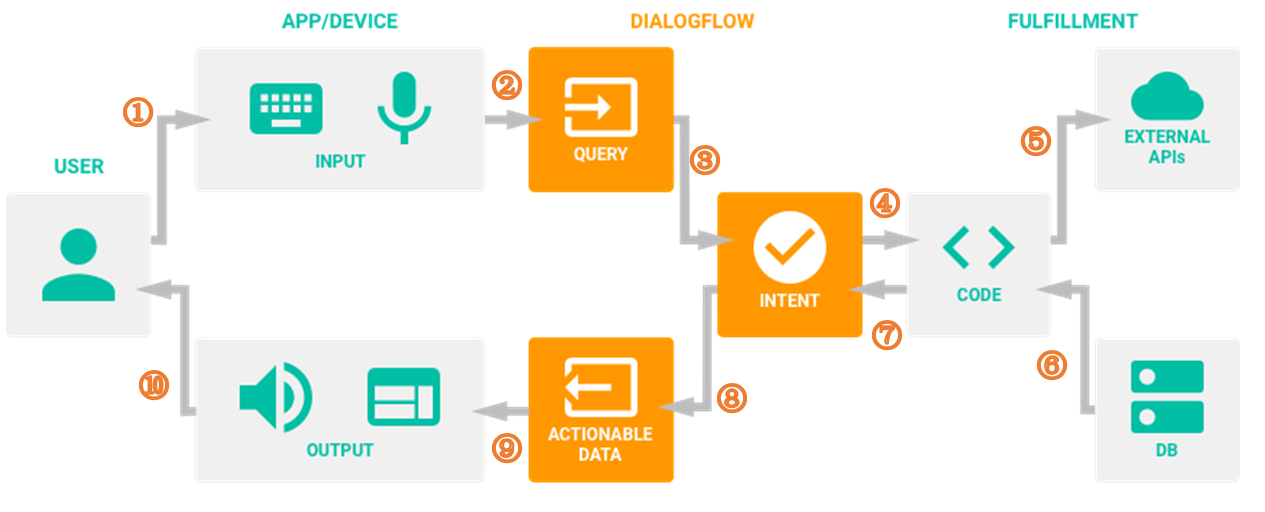
\includegraphics[width=\textwidth,keepaspectratio]{pic/df-overview.jpg}
  \end{center}
  \caption{ภาพรวมการทำงานของ Dialogflow}
  \label{fig:df-overview}
\end{figure}
หลังจากที่ได้ intent มาแล้ว Dialogflow ก็จะทำการเทียบ intent เข้ากับ intent ทั้งหมดที่มีเพื่อหาคำตอบที่ตรงกันที่สุด
เพื่อจะหาว่าผู้ใช้ถามเข้ามาว่าอะไรและควรจะตอบอย่างไรกลับไป
ถ้ามีข้อมูลเพียงพอก็จะตอบกลับไปเลย แต่ถ้าต้องการข้อมูลเพิ่มเติมเช่น ข้อมูลจาก database หรือจาก API อื่นๆก็จะต้องขอ
user request ไปยัง daatabase หรือ API เป้าหมายเพื่อทำ Fulfillment หรือก็คือการเติมเต็มคำตอบและคอยตอบกลับไป
เป็น agent response ให้ กับ user อีกที



\section {Algorithm}
\subsection{Natural Language Processing}
Natural Language Processing หรือ NLP คือ กระบวนการที่ทำให้คอมพิวเตอร์สามารเข้าใจภาษามนุษย์ได้
กระบวนการนี้จะช่วยทำให้คอมพิวเตอร์มีความเข้าใจเกี่ยวกับภาษาที่เราพิมพ์ และยังสามารถตีความจากข้อความได้
ซึ่ง NLP มี subset อยู่ภายในคือ Natural Language Understanding (NLU) โดยจะเน้นการทำงานไปที่ให้คอมพิวเตอร์
ให้สามารถเข้าใจข้อความจากมนุษย์ได้ลึกซึ้งขึ้น โดยฟังก์ชันหลักของ NLU จะมุ่งเน้นหาความสัมพันธ์เชิงความหมายของคำในประโยค,
ดึงใจความสำคัญจากประโยค, เน้นการถามตอบข้อมูลเพิ่มเติม, และเน้นการตอบโต้พูดคุย โดย NLU ถือเป็นหนึ่งในหลักการสำคัญสำหรับ
การทำงานของ Chatbot

\begin{figure}[hbt!]
  \begin{center}
    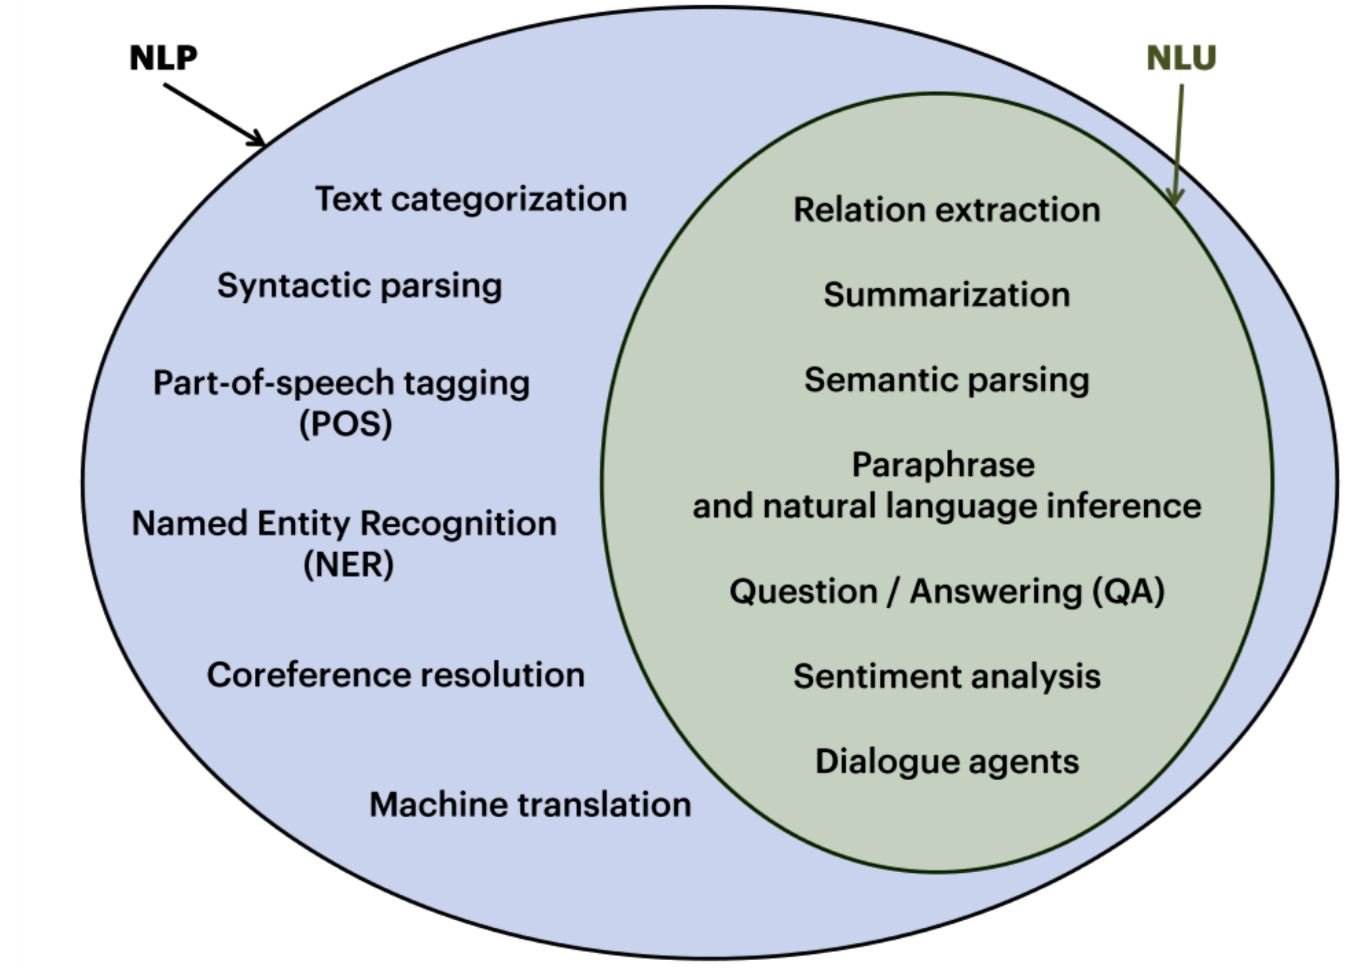
\includegraphics[width=\textwidth,keepaspectratio]{pic/NLPandNUL.png}
  \end{center}
  \caption{Natural Language Processing (NLP) และ Natural Language Understanding (NUL)}
  \label{fig:NLPandNUL}
\end{figure}


\chapter{\ifproject%
\ifenglish Experimentation and Results\else การทดลองและผลลัพธ์\fi
\else%
\ifenglish System Evaluation\else การประเมินระบบ\fi
\fi}

ในบทนี้จะกล่าวที่ผลลัพธ์ของโครงงานเมื่อสร้างเสร็จและฟังก์ชันการทำ หลักๆ จะมีการเทรนบอทให้มี
การตอบที่เป็นธรรมชาติ และมีความแม่นยำถูกต้องในการตอบ ตลอดจนไปถึงความพึงพอใจของผู้ใช้งาน
\section{การประเมินประสิทธิภาพ (Performance evaluation)}
สามารถจำแบบออกเป็น 3 หัวข้อดังนี้
\subsection{ความถูกต้องในการตอบคำถาม (Accuracy)} 
โดยจะจัดทำ trining data set สำหรับการทดสอบและบันทึกผลโดยมีเป้าหมายคือมีความแม่ยำมากกว่า 85\% ขึ้นไป

\subsection{ความรวดเร็วในการทำงาน (Response time)}
โดยจะทำการทดลองส่ง request ไปยังตัว Dialogflow และวัดเวลาในการตอบกลับโดยใช้ JMeter ซึ่งเป็นเครื่องมือสำหรับวัด
ประสิทธิภาพของ software บันทึกผลและปรับปรุงการทำงาน

\section{ความพึงพอใจของผู้ใช้งาน (User Satisfaction)}
จะจัดทำแบบสอบถามสำหรับผู้ที่ใช้งานสำรวจความคิดเห็นว่าผู้ใช้งานโดยจะแบ่งออกเป็น 5 หัวข้อดังนี้
\begin{enumerate}
    \item มีความพึงพอใจหรือไม่
    \item พึงพอใจในส่วนใดเป็นพิเศษ
    \item ไม่พึ่งพอใจในส่วนใด
    \item อยากเพิ่มอะไรเข้าไปไหม
    \item ความแม่นยำเป็นอย่างไร 
\end{enumerate}





\ifproject
\chapter{\ifenglish Conclusions and Discussions\else บทสรุปและข้อเสนอแนะ\fi}

\section{\ifenglish Conclusions\else สรุปผล\fi}

โครงงานนี้เป็นโครงการที่ใช้การพัฒนาแชทบอทผ่าน Dialogflow โดยเชื่อมต่อกับ Web application ด้วย NodeJS และใช้ Firebase
ในการจัดเก็บข้อมูลและสื่อสารกับ Dialogflow โดยโครงงานนี้สามารถตอบคำถามได้ถูกต้องมากกว่า 85\% และมีความแม่นยำอยู่ที่ 86.66\%
โดยเวลาในการตอบคำถามเฉลี่ยอยู่ที่ 1.911 วินาที โครงงานนี้ยังสามารถอัพโหลดวิดีโอและเชื่อมต่อกับ API จาก Cutt.ly, IQAir และ
OpenWeatherMap ได้ โดยโครงงานนี้เป็นตัวอย่างที่ดีของการใช้ Dialogflow และ Firebase
ในการสร้างแชทบอทที่มีประสิทธิภาพและเป็นประโยชน์แก่ผู้ใช้งานที่เข้ามาใช้บริการ

\section{\ifenglish Challenges\else ปัญหาที่พบและแนวทางการแก้ไข\fi}

หลังจากทำการทดสอบโครงงานนี้ พบว่ามีปัญหาบางอย่างเกี่ยวกับการตอบคำถามที่ไม่ถูกต้อง
และความเร็วในการตอบคำถามที่อาจจะช้าไปบ้าง ดังนั้นเราสามารถแก้ไขปัญหาดังกล่าวได้โดยการ:
\begin{enumerate}
  \item ปรับปรุงโมเดลตัวช่วยเติมคำศัพท์ (autocomplete) ให้มีความแม่นยำและครอบคลุมคำศัพท์มากขึ้น เพื่อลดปัญหาการตอบคำถามที่ไม่ถูกต้อง
  \item ปรับแต่งโครงสร้างของระบบเพื่อเพิ่มประสิทธิภาพในการตอบคำถาม และลดความช้าในการตอบคำถาม
  \item พัฒนาระบบให้สามารถรับรู้ได้ว่าผู้ใช้งานได้เข้าใจคำตอบหรือยัง และจะสามารถแนะนำคำตอบที่เหมาะสมกับคำถามได้ในกรณีที่ตอบไม่ถูกต้อง
  \item พัฒนาระบบให้สามารถตรวจสอบความถูกต้องของคำตอบก่อนส่งคำตอบกลับไปยังผู้ใช้งาน และแสดงข้อความแจ้งเตือนในกรณีที่ตอบไม่ถูกต้อง
  \item ปรับปรุงเทคโนโลยีการแปลงคำพูดเป็นข้อความและการแปลงข้อความเป็นเสียงเพื่อเพิ่มความแม่นยำในการตอบคำถามและลดความล่าช้าในการตอบคำถาม
  \item ปรับปรุงการจัดการฐานข้อมูลในการเก็บคำถามและคำตอบ เพื่อให้สามารถค้นหาและดึงข้อมูล
\end{enumerate}


\section{\ifenglish%
Suggestions and further improvements
\else%
ข้อเสนอแนะและแนวทางการพัฒนาต่อ
\fi
}

ข้อเสนอแนะเพื่อพัฒนาโครงงานนี้ต่อไป มีดังนี้
\begin{enumerate}
  \item พัฒนาการตอบคำถามที่สามารถตอบได้มากกว่า 85\%: โดยการทำการเพิ่มข้อมูลให้กับ Dialogflow เพื่อเพิ่มความแม่นยำในการตอบคำถาม และสามารถใช้ Machine Learning ในการปรับปรุงความแม่นยำในการตอบคำถามได้เช่นกัน
  \item พัฒนาฟังก์ชันการสื่อสารที่ดีขึ้น: โดยการเพิ่มฟังก์ชันเสียงเพื่อให้ผู้ใช้งานสามารถใช้งานได้ง่ายขึ้น และเพิ่มความสามารถในการรับรู้เสียงและสื่อสารที่ดีขึ้น
  \item พัฒนาการเชื่อมต่อกับฐานข้อมูลที่ดีขึ้น: โดยการเพิ่มฟังก์ชันการเชื่อมต่อกับฐานข้อมูลแบบ NoSQL หรือ SQL เพื่อทำให้การจัดการข้อมูลง่ายขึ้นและทำให้ระบบทำงานได้รวดเร็วขึ้น
  \item พัฒนาการตรวจสอบความถูกต้องของข้อมูล: โดยการเพิ่มฟังก์ชันการตรวจสอบความถูกต้องของข้อมูลที่ผู้ใช้งานให้มา และแสดงข้อความแจ้งเตือนเมื่อมีข้อมูลที่ไม่ถูกต้อง
  \item พัฒนาระบบการทดสอบและการตรวจสอบความเสถียร: โดยการเพิ่มฟังก์ชันการทดสอบและการตรวจสอบความเสถียรในระบบ เพื่อให้ระบบทำงานได้ถูกต้องและไม่เกิดข้อผิดพลาดใดๆ ที่อาจจะเกิดขึ้นในอนาคต
\end{enumerate}
\fi

\bibliography{myReport}

\ifproject
\normalspacing
\appendix

\chapter{การ setup firebase}

การตั้งค่า Firebase สำหรับโครงการนี้ ประกอบด้วยการตั้งค่า Firebase Realtime Database และ Firebase Storage
เพื่อทำการเก็บข้อมูลที่สำคัญของโปรแกรม

\section{สร้างโปรเจ็กต์ใน Firebase Console}
\begin{enumerate}
\item ไปที่ \url{https://console.firebase.google.com/} แล้วเข้าสู่ระบบด้วยบัญชี Google ของคุณ
\item เข้าไปที่ Firebase Console และคลิกที่ปุ่ม "Add project" เพื่อสร้างโปรเจ็กต์ใหม่
\item ตั้งชื่อโปรเจ็กต์และเลือกประเทศที่คุณอยู่
\item เปิดใช้งาน Google Analytics หากต้องการ
\item กดปุ่ม "Create project" เพื่อสร้างโปรเจ็กต์ใหม่
\end{enumerate}

\section{เปิดใช้งาน Firebase Realtime Database}
\begin{enumerate}
\item เลือก "Realtime Database" จากเมนูด้านซ้ายของ Firebase Console
\item กดปุ่ม "Create Database" และเลือกโหมด "Start in test mode"
\item บันทึกการตั้งค่า
\end{enumerate}

\section{เปิดใช้งาน Firebase Storage}
\begin{enumerate}
\item เลือก "Storage" จากเมนูด้านซ้ายของ Firebase Console
\item กดปุ่ม "Get started" เพื่อเริ่มต้นการตั้งค่า
\item เลือกโปรไฟล์ของโปรเจ็กต์
\item เลือกโฟลเดอร์เริ่มต้นเพื่อเก็บไฟล์
\item เลือก "Start upload" เพื่ออัปโหลดไฟล์
\end{enumerate}
มีตัว bot สำหรับ upload video ให้ในไฟล์ \verb+Google_Cloud_Function/localBot.py+ สามารถอ่านวิธีการใช้งานได้จาก
\url{https://github.com/mekkkwiz/Speech-Navigation-Chatbot/blob/master/Google_Cloud_Function/README.md}

\section{เพิ่มคีย์การเข้าถึงของ Firebase ในโปรเจกต์ของเรา}
\begin{enumerate}
\item ไปที่หน้า Console Firebase แล้วเลือกโปรเจกต์ที่เราสร้างไว้
\item เลือกเมนู Setting (icon รูปแฮมเบอร์เกอร์) จากด้านบนขวามือของหน้าจอ
\item คลิกที่โปรเจกต์ของเราแล้วเลือกแท็บ Service Accounts จากนั้นคลิก Generate New Private Key
\item ไฟล์ key จะถูกดาวน์โหลดลงบนเครื่องคุณ ให้เก็บไฟล์ key นี้ไว้ในโฟลเดอร์ DfFulfillment ของโปรเจกต์
\item เปลี่ยนชื่อไฟล์ key ให้เป็น serviceAccountKey.json
\end{enumerate}

\chapter{\ifenglish Manual\else คู่มือการใช้งานระบบ\fi}


\section{การติดตั้ง}
\begin{enumerate}
\item ดาวน์โหลด repository จาก \url{https://github.com/mekkkwiz/Speech-Navigation-Chatbot}
\item เปิด Command Prompt หรือ Terminal แล้วเข้าไปยังโฟลเดอร์ final-project-app ที่ดาวน์โหลดมา
\item ใช้คำสั่ง npm install เพื่อติดตั้ง dependencies ทั้งหมด
\item เข้าไปยังโฟลเดอร์ \verb+client_v2+ แล้วใช้คำสั่ง npm install เพื่อติดตั้ง dependencies ที่เกี่ยวข้อง
\item เข้าไปยังโฟลเดอร์ DfFulfillment แล้วใช้คำสั่ง npm install เพื่อติดตั้ง dependencies ที่เกี่ยวข้อง
\item สร้างไฟล์ .env และกำหนดค่าตัวแปรต่างๆดังนี้
\begin{verbatim}
GOOGLE_PROJECT_ID="your-project-id"
DIALOGFLOW_SESSION_ID="unique-session-id"
DIALOGFLOW_SESSION_LANGUAGE_CODE="th"
GOOGLE_CLIENT_EMAIL="your-client-email"
GOOGLE_PRIVATE_KEY="your-private-key"
\end{verbatim}
และดาวน์โหลด service account key จาก Google Cloud Platform แล้วบันทึกเป็นไฟล์
serviceAccountKey.json ในโฟลเดอร์ DFfullfillment ของโปรเจค
\end{enumerate}
\section{การ start server}

\begin{enumerate}
\item เปิด Terminal แล้วเข้าไปยังโฟลเดอร์ final-project-app ที่ดาวน์โหลดมา
\item ใช้คำสั่ง npm run dev เพื่อเริ่มต้นเซิร์ฟเวอร์
\item เปิด Terminal อีกหนึ่งหน้าแล้วเข้าไปยังโฟลเดอร์ DfFulfillment ใช้คำสั่ง npm run dev เพื่อเริ่มต้น Fulfillment Server
\item คุณอาจต้องใช้ ngrok เพื่อให้เซิร์ฟเวอร์ของ Fulfillment Server สามารถเข้าถึงจาก internet ได้ โดยดาวน์โหลดจาก \url{https://ngrok.com/download} แล้วใช้คำสั่ง ngrok http 3030 เพื่อเปิด ngrok
\item คัดลอก https url ที่ได้จาก ngrok เข้าไปไว้ใน fulfillment url ในเว็บ dialogflow
\end{enumerate}

\section{การใช้งาน}
\begin{enumerate}
\item เปิดโปรแกรมในเบราว์เซอร์โดยไปที่ \url{http://localhost:3000}
\item อนุญาตการเข้าถึงไมโครโฟนของคุณ
\item ใช้คำสั่งด้วยเสียงเพื่อนำทางในอาคาร สอบถามตำแหน่งของอาจารย์ หรือสอบถามเรื่องสภาพอากาศ
\item โปรแกรมจะตอบกลับด้วยเสียงผ่าน Google TTS API
\end{enumerate}

\section{วิธีการติดตั้งเพิ่มเติม}
สามารถอ่านวิธีการติดตั้งเพิ่มเติมได้ที่
\\\url{https://github.com/mekkkwiz/Speech-Navigation-Chatbot}


%% Display glossary (optional) -- need glossary option.
\ifglossary\glossarypage\fi

%% Display index (optional) -- need idx option.
\ifindex\indexpage\fi

\begin{biosketch}
\begin{center}
  \includegraphics[width=1.5in]{mugshot.jpg}
\end{center}
Your biosketch goes here. Make sure it sits inside
the \texttt{biosketch} environment.
\end{biosketch}
\fi % \ifproject
\end{document}
